\documentclass[12pt]{article}
\usepackage{HomeWorkTemplate}
\usepackage{circuitikz}
\usepackage[shortlabels]{enumitem}
\usepackage{hyperref}
\usepackage{tikz}
\usepackage{xepersian}
\usepackage{graphicx}
\usetikzlibrary{arrows,automata}
\usetikzlibrary{circuits.logic.US}
\settextfont{XB Niloofar.ttf}
\usepackage{changepage}
\newcounter{problemcounter}
\newcounter{subproblemcounter}
\setcounter{problemcounter}{1}
\setcounter{subproblemcounter}{1}
\newcommand{\problem}[1]
{
	\subsection*{
		پرسش
		\arabic{problemcounter} 
		\stepcounter{problemcounter}
		\setcounter{subproblemcounter}{1}
		#1
	}
}
\newcommand{\subproblem}{
	\textbf{\harfi{subproblemcounter})}\stepcounter{subproblemcounter}
}



\begin{document}

\handout
{نظریه زبان‌‌ها و اتوماتا}
{تمرین سری یک}
{امیررضا اکبری}
{۱۱۱۱۱۱۱۱}
{}
\problem{}
\subproblem{}
 به سادگی مشخص است که این عبارت غلط است زیرا شخصی که از این رستوران سفارش داده است یا از قبل سفارش داده بوده
 که به وضوح راضی بود و مشتری رستوران است و نظر ان مثبت و در غیر این صورت این شخص از طرف شخصی دیگر
 که سلیقه های مشابهی دارند معرفی شده یا خودش در نگاه اول از رستوران راضی بوده که این رستوران را برای سفارش انتخاب کرده
 و در کل تعداد حالات کمی وجود دارد که شخص نظر منفی داشته باشد و این نمونه گیری به وضوح اریب است.
\newline
\subproblem{} 
این نمونه گیری نیز به دلایل مختلفی که چند نمونه را ذکر خواهم کرد اریب است. یکی اینکه ریاضی دو درسی پایه و اجباری است.
یکی دیگر اینکه درس فلسفه ریاضی فقط مربوط به دانشکده ریاضی و همجین درس اختیاری است در صورتی که 
ریاضی دو مربوط به کل دانشگاه و اجباری است.
یکی دیگر از دلایل این است که برای خیلی از دانشجویان نمره خوب را به سادگی گرفتن ملاک است ولی دکتر شهشهانی استادی
سخت گیر است.
\problem{}
\subproblem{}
از لحاظ مفهومی چولگی به معنای میزان دوری داده های پرت است یا به عبارتی
علامت آن نشان دهنده راست یا چپ بودن داده های دور تر از میانگین یا مد است.
\newline
\subproblem{}
با توجه به ضریب چولگی اول پیرسن ($\frac{\bar{x} - M}{s} $) چپ بودن چولگی به معنای منفی بودن این عبارت و درنتیجه بزگ تر بودن مد از میانگین است.
\newline 
   منفی بودن این عبارت نشان دهنده بزرگ تر بودن میانه نسبت به میانگین است. ($\frac{3(\bar{x} - m)}{s} $) از طرف دیگر با توجه به ضریب چولگی دوم پیرسن 
\newline
  پس کافیست نشان دهیم رابطه بین مد و میانه چگونه است از طرف دیگر با توجه به ضریب چولگی گشتاوری منفی بودن چولگی به معنی وجود داده بیشتر داده های دور تر از میانگین در سمت چپ میانگین است که
این به معنی بزرگ تر بودن بازه 
\newline
\subproblem{}
برابر بودن ضریب اول و دوم پیرسن به ما رابطه زیر را می دهنده
\newline
$\frac{\bar{x} - M}{s} $ = $\frac{3(\bar{x} - m)}{s} $ = 0.32
\newline
 که با قرار دادن میانگین و انحراف معیار به ترتیب داریم:
 \newline
 $\frac{29.6 - M}{6.5} = 0.32 $\newline
 $ M = 27.52$ : مد
 \newline
 $\frac{3(29.6 - m)}{6.5} = 0.32 $\newline
 $29.6 - m = 0.693$\newline
 $m = 28.9 $ تقریباااااا
\problem{}
\subproblem{}
\begin{figure}[h]
	\centering
	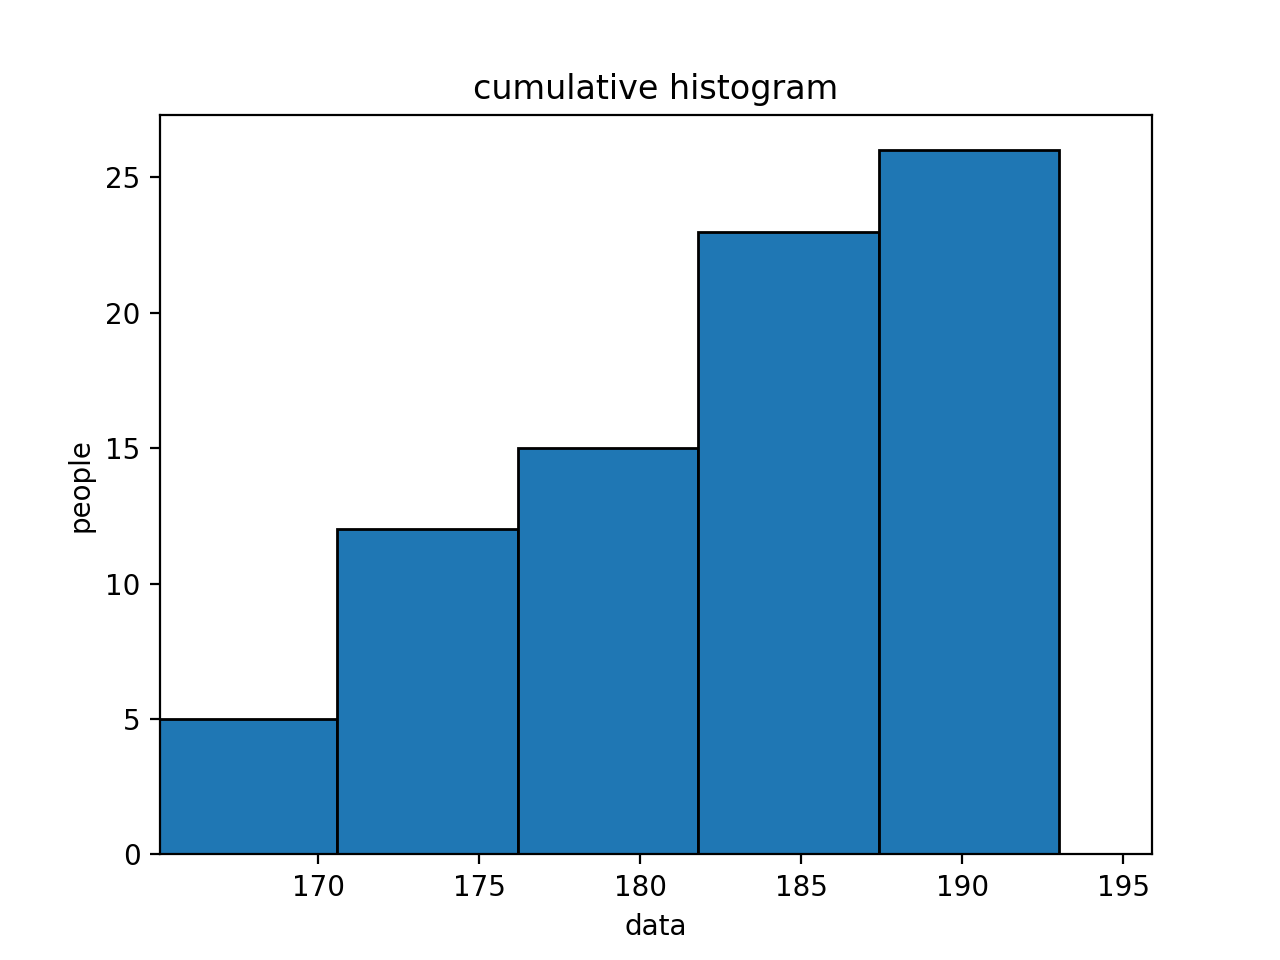
\includegraphics[width=0.5\textwidth]{Figure_1.png}
	\caption{نمودار توزیع تجمعی رسم شده توسط python}
	\label{fig:my_label}
  \end{figure}
\problem{}
\problem{}
\problem{}
\problem{}
\end{document}